\section{Модификация проекта «Выпуклая оболочка»}
\subsection{Постановка задачи}

Модифицируйте эталонный проект таким образом, чтобы вычислялась мощность 
множества точек пересечения границы выпуклой оболочки 
с замкнутым единичным кругом с центром в начале координат.

После запуска программа предлагает пользователю ввести последовательно 
координаты вершин выпуклой оболочки. Введённая точка индуктивно 
добавляется в выпуклую оболочку. Нам же необходимо вместе со 
значениями периметра и площади выпуклой оболочки выводить мощность 
множества точек пересечения границы выпуклой оболочки 
с замкнутым единичным кругом с центром в начале координат.

Допустим для точек $A(-1,-1)$, $B(1,1)$ и $C(1,-1)$ программа выдаст 
в качестве ответа \verb|infinity|, потому что отрезок $AB$ 
пересекает единичный круг в бесконечном множестве точек, но при 
добавлении точки $D(-1,1)$ множество перевычисляется, и в качестве ответа 
выдаётся \verb|4|, потому что квадрат $ABCD$ описывает окружность и 
пересекается с ней в четырёх точках.

\subsection{Решение и модификация кода}

Для решения данной задачи нам необходимо находить расстояние от центра 
круга до стороны выпуклой оболочки. Это задание сводится к нахождения 
расстояния от точки до отрезка(точка нам задана $O(0,0)$, а отрезком 
является сторона выпуклой оболочки).

Допустим нам дан отрезок $AB$ и точка $O$. Расстоянием от точки $O$ 
до отрезка $AB$ является отрезок $OA$, $OB$ или высота из точки $O$ 
до $AB$(если эта высота падает на $AB$). Высота падает 
на $AB$, если $\angle OAB$ и $\angle OBA$ являются острыми или 
один из них прямой, другой острый. Нам даны лишь координаты этих точек. 
С помощью метода \verb|dist| класса \verb|R2Point| можно найти 
расстояние всех трёх сторон. Затем по теореме косинусов находим 
$\cos\angle A$ и $\cos\angle B$:
$$OB^2 = AO^2+AB^2-2\cdot AO\cdot AB\cos\angle A \Rightarrow 
\cos\angle A = \frac{AO^2+AB^2-OB^2}{2\cdot AO\cdot AB}$$

Аналогично находим $\cos\angle B$. Затем определяем -- является 
ли угол острым или прямым. Если выполняется условие: 
$0 \leqslant \cos\alpha \leqslant 1$, то угол острый или прямой. 
Саму высоту мы находим из площади треугольника: $S=\frac12\cdot 
AB\cdot h \Rightarrow h=\frac{2\cdot S}{AB}$. Сторона $AB$ известна, 
площадь можно найти с помощью метода \verb|R2Point.area| 
класса \verb|R2Point|.

Теперь можно найти растояние от точки до стороны выпуклой оболочки, 
как наименьшее значение длины среди сторон $AO$, $OB$ и $h$.

\newpage

После этого можно найти множество точек пересечения отрезка с 
замкнутым единичным кругом в начале координат. Если расстояние меньше 
единицы, то множеством точек пересечения будет являться 
\verb|infinity|(рис.~\ref{fig:ro_0}):
\begin{figure}[ht!]
\begin{center}
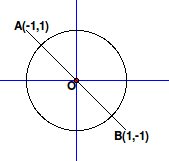
\includegraphics[scale=0.6]{images/ro_0}
\end{center}
\vspace*{-8mm}
\caption{}\label{fig:ro_0}
\end{figure}

Если расстояние равно единицы, то множеством точек пересечения будет 
являться \verb|1|(рис.~\ref{fig:ro_1}):
\begin{figure}[ht!]
\begin{center}
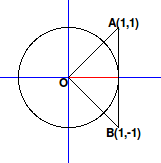
\includegraphics[scale=0.6]{images/ro_1}
\end{center}
\vspace*{-8mm}
\caption{}\label{fig:ro_1}
\end{figure}

Если расстояние больше единицы, то множеством точек пересечения будет 
являться \verb|0|(рис.~\ref{fig:ro_more}):
\begin{figure}[ht!]
\begin{center}
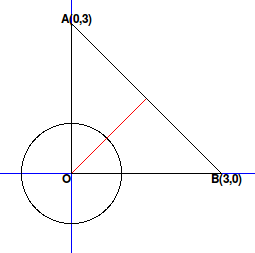
\includegraphics[scale=0.45]{images/ro_more}
\end{center}
\vspace*{-8mm}
\caption{}\label{fig:ro_more}
\end{figure}

Метод \verb|R2Point.intersect|, который принимает две точки в качестве 
аргумента и выдаёт множество точек пересечения этого отрезка с 
единичным кругом описан в классе \verb|R2Point| и реализован 
следующим образом:
\begin{small}
\verbatiminput{programms/multi.rb}
\end{small}

Теперь можно находить множество точек пересечения стороны выпуклой 
оболочки с кругом. Рассмотрим это вычисление для всей выпуклой оболочки.

Если выпуклой оболочкой является точка, то множество точек 
пересечения с кругом будет сама эта точка, либо множество будет 
равняться нулю. Для отрезка мы уже знаем как найти это множество, 
а многоугольник рассмотрим подробно.

Так как ответом пересечения стороны выпуклой оболочки и круга 
может быть число или \verb|infinity|, то целесообразно хранить сумму 
этих чисел(\verb|@n_point|), количество 
\verb|infinity|(\verb|@n_infinity|) и итоговый ответ(\verb|@n_points|) 
в разных переменных. Для того, чтобы менять значения этих переменных 
в зависимости от удаления или добавления ребра выпуклой оболочки, 
написан метод \verb|oper_with_n_p|, принимающий на вход две точки для 
отрезка и ещё один аргумент, позволяющий обрабатывать ситуацию, когда 
ребро выпуклой оболочки удаляется или добавляется. Этот метод 
находится в секции \verb|private| для того, чтобы он был виден 
только в классе \verb|Polygon|. Листинг данного метода:
\begin{small}
\verbatiminput{programms/oper.rb}
\end{small}

Теперь с помощью этого метода можно индуктивно вычислять множество 
точек пересечения замкнутого круга с центром в начале координат.

При добавлении новой точки необходимо учитывать удаление освещенных 
рёбер, соответственно мощность множества точек пересечения необходимо 
пересчитывать. Чтобы сделать это индуктивно, мы используем дек, в 
который помещаем значение точек -- вершин выпуклой оболочки.

Сам процесс индуктивного перевычсления мощности множества точек 
пересечнения можно представить в таблице(табл.~\ref{tab:tab1}), которая приведена ниже:
\begin{table}[h!]
\begin{tabular}{|p{6cm}|p{10cm}|}
\hline
Удаляем ребро, соединяю-
щее начало и конец дека,
если оно освещено нашей
точкой:
&
\verb|oper_with_n_p(@points.last,@points.first,"del")|\\
\hline
Удаляем освещенные реб-
ра из начала дека:
&
\verb|oper_with_n_p(p, @points.first, "del")|\\
\hline
Удаляем освещенные реб-
ра из конца дека:
&
\verb|oper_with_n_p(p, @points.last, "del")|\\
\hline
Обрабатываем два добавленных ребра:
&
\verb|oper_with_n_p(t, @points.first)|
\verb|oper_with_n_p(t, @points.last)|\\
\hline
\end{tabular}
\caption{}\label{tab:tab1}
\end{table}

Пример работы программы представлен на рис.~\ref{fig:ex1}. 
Добавляются точки ABC и результат: \verb|infinity|. Затем добавляется 
точка D(рис.~\ref{fig:ex2}), множество точек пересчитывается и 
результатом будет число $4$ -- четыре точки пересечения выпуклой 
оболочки с кругом.
\begin{figure}[ht!]
\begin{center}
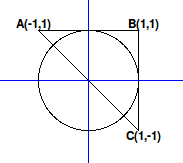
\includegraphics[scale=0.6]{images/circ}
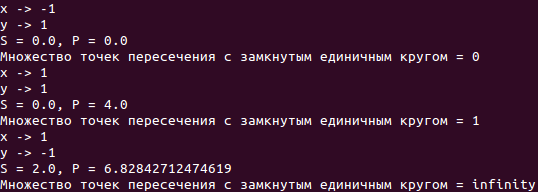
\includegraphics[scale=0.5]{images/ex1}
\end{center}
\vspace*{-8mm}
\caption{}\label{fig:ex1}
\end{figure}

\begin{figure}[ht!]
\begin{center}
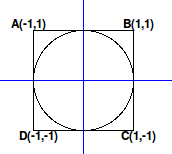
\includegraphics[scale=0.6]{images/circ2}
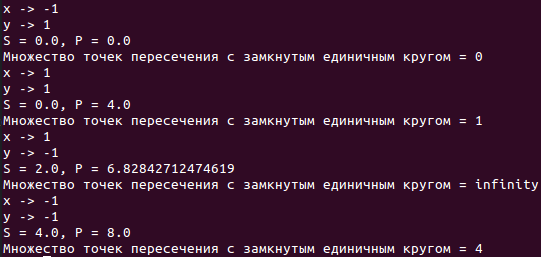
\includegraphics[scale=0.4]{images/ex2}
\end{center}
\vspace*{-8mm}
\caption{}\label{fig:ex2}
\end{figure}
